Die folgenden Kapitel geben einen Überblick über die verwendeten Technologien während der Bachelorarbeit liefern. Sie sollen auch Aufschluss darüber geben, wieso diese verwendet wurden und welche Vorteile sie besitzen. Zuerst wird in Kapitel \ref{sec:R} die Programmiersprache R und deren Entwicklungsumgebung RStudio erklärt, um im Anschluss in Kapitel \ref{sec:Rcpp} die Vorzüge vom Paket \emph{Rcpp} und die dabei verwendete Sprache C++ zu beschreiben. Am Ende wird in Kapitel \ref{sec:RMarkdown} über die Visualisierungsmöglichkeiten gesprochen, die dem Studenten helfen soll, die Abläufe des Turbo-Kode-Verfahrens besser zu verstehen. Dabei wird die Auszeichnungssprache \emph{RMarkdown} und die darin verwendeten Sprachkonstrukte näher erläutert.

\section{R, RStudio, Pakete}
\label{sec:R}
Die Programmiersprache R wurde 1992 von den beiden Statistikern  Ross Ihaka und Robert Gentleman an der Universität Auckland entwickelt. Dabei wurde die Sprache speziell für Anwendungsfälle im statistischen Bereich gebaut. Die Sprache baut auf den Vorgänger S auf und wird mit einen Kommandozeileninterpreter ausgeliefert. Dadurch dass der Quellcode nicht kompiliert, sondern nur interpretiert wird, ist er auf verschiedenen Plattformen ausführbar. Der kanadische Mitentwickler John M. Chambers beschreibt die Sprache folgenderweise:

\enquote{To understand computations in R, two slogans are helpful: Everything that exists is an object. Everything that happens is a function call.} \cite{chambers2014object}\\

Diese beiden Aussagen beschreiben, dass R nur aus Objekte und Funktionen besteht. Das bedeutet, dass jede Variable ein Objekt ist, das zur Laufzeit seine Struktur verändern kann. Somit ist R eine schwach, dynamisch typisierte Programmiersprache. Dadurch muss einer Variable kein Datentyp zugewiesen werden und die Typüberprüfung findet erst zur Laufzeit statt. Ein weiterer Grund R zu verwenden, ist die hervorragende Eigenschaft, große Datenmengen graphisch darzustellen. Dieses Problem lässt sich mit R hervorragend bewältigen.

Um den Funktionsumfang der Sprache zu erweitern, stehen zahlreiche Pakete auf den CRAN-Servern\footnote{The Comprehensive R Archive Network: \url{https://cran.r-project.org/}} zur Verfügung. Dort veröffentlicht die R-Community ihre entwickelten Pakete, um sie mit den restlichen Nutzern von R zu teilen. Damit ein selber entwickeltes Paket dort aufgenommen wird, muss es strenge Kriterien erfüllen, um die Qualität der Pakete zu sichern. Mittlerweile stehen über 8000 verschiedene Pakete (Stand: Mai 2016) auf den Servern zum Download bereit. Diese decken einen großen Anwendungsbereich ab und sind daher sehr hilfreich, um selbst R-Code zu entwickeln\cite{rmanual}.

Zwei sehr wichtige Pakete sind notwendig, um selbst R-Pakete zu entwickeln. Dazu zählt \emph{devtools}, das hilfreiche Funktionen für die Erstellung (Build) von Paketen zur Verfügung stellt. Damit werden viele Tätigkeiten automatisiert, die ansonsten vom Entwickler getätigt werden müssen \cite{devtools}.

Ein weiteres wichtiges Paket zur Unterstützung bei der Entwicklung eines Paketes ist \emph{roxygen2}. Damit lässt sich ähnlich wie bei \emph{JavaDoc}, Kommentare in den Quellcode schreiben, die dann automatisch zu einer Paketdokumentation führen. Die \emph{roxygen2}-Kommentare starten mit \# '. Die wichtigsten Annotation sind für die Parameter (@param) und für den Rückgabewert (@return). Es können auch Beispiele (@examples) eingebunden werden, die dann automatisch bei der Erstellung getestet werden, ob sie richtig funktionieren. Wahrscheinlich die wichtigste Annotation bei der Entwicklung ist die Veröffentlichung einer Funktion im Paket (@export), dadurch wird sichergestellt, dass der Benutzer Zugriff zu dieser Funktion hat \cite{roxygen}.

\begin{figure}[t]
\centering
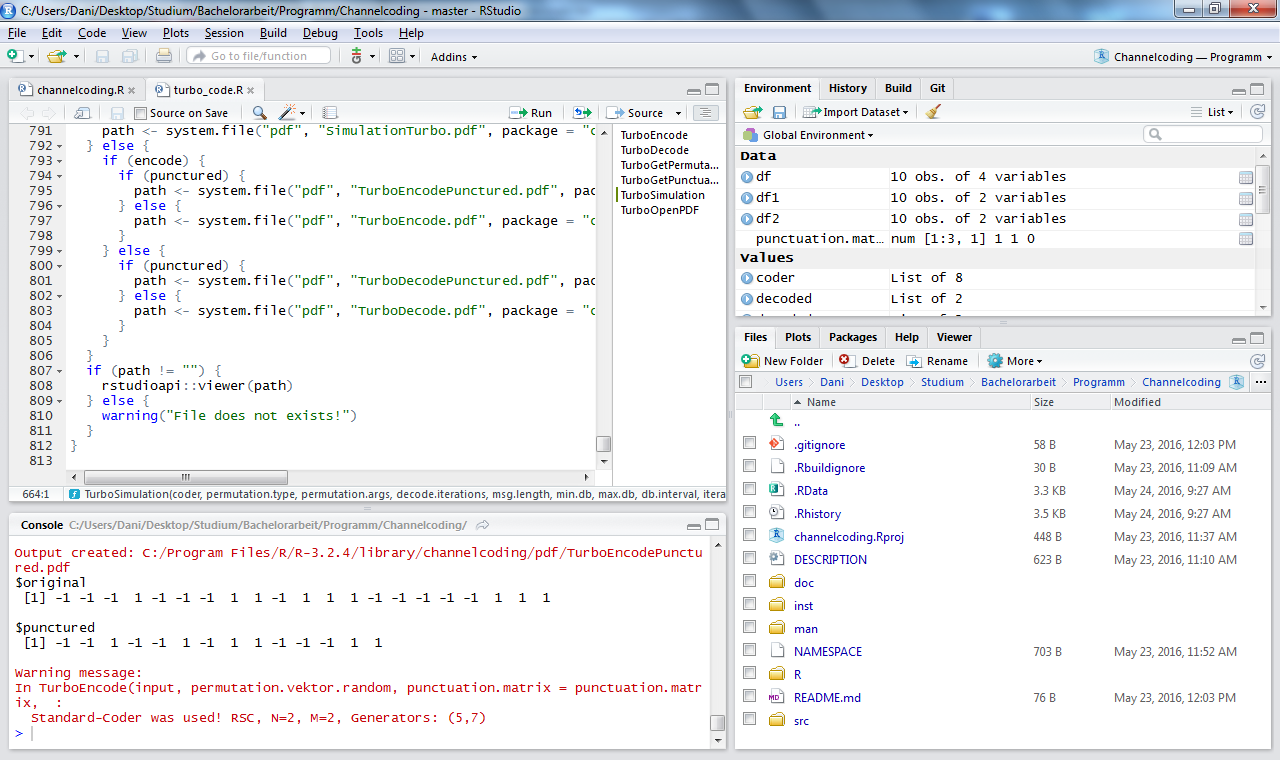
\includegraphics[width=\ScaleIfNeeded]{pictures/RStudio}
\caption{RStudio Standartansicht}
\label{pic:RStudio}
\end{figure}

Die weitverbreiteste Entwicklungsumgebung für die Programmiersprache R ist das RStudio, das in der Abbildung \ref{pic:RStudio} zu sehen ist. Diese Umgebung wurde speziell für den Softwareentwurf mittels R entwickelt und stellt alle wichtigen Funktionen zur Verfügung. Damit ist es besonders einfach selber R-Pakete zu entwickeln, oder andere Programmiersprachen mittels speziellen Schnittstellen mit R zu verbinden. Zur Visualisierung von den Berechnungsergebnissen sind bereits einige Vorlagen in die Entwicklungsumgebung integriert. Zum Beispiel ist es sehr einfach HTML Seiten, PDF Dokumente oder auch interaktive Oberflächen mittels \emph{Shiny} zu erstellen. Um dynamische Dokumente zu erstellen kann auch \emph{RMarkdown} verwendet werden, das wird in Kapitel \ref{sec:RMarkdown} näher erklärt.

\section{C++, Rcpp}
\label{sec:Rcpp}
Die Performanz von R ist bei der Verwendung von Schleifen relativ schlecht. Aufgrund der schwachen Typisierung, muss die Implementierung der Schleife für jeden Datentyp funktionieren, dadurch wird die Geschwindigkeit wesentlich reduziert. Darum kann man bei einer intensiven Nutzung von Schleifen auf C oder C++ zurückgreifen und mit einer speziellen Schnittstelle diesen Code von R aufrufen.

Grundsätzlich gibt es drei Möglichkeiten C/C++-Code von R aufzurufen:
\begin{itemize}
	\item \emph{.C} native Schnittstelle
	\item \emph{.Call} Schnittstelle
	\item \emph{Rcpp} Paket
\end{itemize}

Bei der ersten Möglichkeit handelt es sich um die einfachste Möglichkeit C-Code in R auszuführen. Dabei hat der C-Code keinerlei Informationen über die R-Datentypen, sondern erhält als Argumente nur Zeiger auf bestimmte Speicherstellen. Als Rückgabe einer Funktion müssen wieder Zeiger verwendet werden, für die bereits im R-Code Speicherplatz reserviert werden musste.

Die \emph{.Call}-Schnittstelle ist eine Erweiterung der \emph{.C}-Schnittstelle. Sie ist wesentlich schwieriger zu verwenden, bietet allerdings einige hilfreiche Features. Zum Beispiel ist es möglich R-Datentypen direkt zu verwenden und auch die Rückgabe eines Wertes an R, kann einfach mit der normalen Rückgabe in einer C-Funktion erfolgen \cite{wickham2015r}.

Die empfohlene Variante mittlerweile ist die Verwendung des Paketes \emph{Rcpp}, weil dadurch der C++-Code übersichtlich bleibt und der Benutzer viele hilfreiche R-Datentypen zur Verfügung hat (Vektoren, Matrizen, Listen, ...). Noch dazu gibt es einige Funktionen die in C++ gleich verwendet werden können wie in R, zum Beispiel ist es möglich der Wurzelfunktion einen ganzen Vektor als Parameter mitzugeben und erhält dann einen Vektor retour, von dem jeder einzelne Wert die Wurzel gezogen wurde. In der STL-Bibliothek sind viele weitere Datenstrukturen und Algorithmen die im C++-Code verwendet werden können und somit das Leben des Programmierers erleichtern können. Durch die gute Integration von \emph{Rcpp} in die Entwicklungsumgebung RStudio ist es sehr einfach bei der Entwicklung von einem Paket C++-Code zu verwenden. Beim Erzeugen des Paketes kompiliert RStudio automatisch alle C++-Dateien und erstellt automatisch Wrapper-Funktionen, die den Zugriff auf die Funktionen erleichtern. Die genaue Verwendung von diesem \emph{Rcpp}-Paket ist im Buch von Hadley Wickham nachzulesen \cite{wickham2015advanced}. 

\section{RMarkdown, \LaTeX, Ti\textit{k}Z}
\label{sec:RMarkdown}
Mittels dem Paket \emph{RMarkdown} lassen sich sehr einfach dynamische Dokumente im RStudio erzeugen. Dabei wird grundsätzlich die Auszeichnungssprache Markdown verwendet, jedoch lassen sich einfach R-, \LaTeX - und HTML-Code in die RMarkdown-Datei (.rmd Dateiendung) integrieren. Dadurch hat man ein flexibles Werkzeug, um personalisierte Dokumente zu erstellen. Das Ausgabeformat kann einfach in den Kopfzeilen der Datei bestimmt werden. Dabei sind folgende Formate möglich: HTML, PDF, Word, RTF, ODT oder einfaches Markdown. Noch dazu ist es sehr einfach eine Präsentation zu erstellen, da mit einfachen Befehlen im Quellcode neue Folien oder Auflistungen erzeugt werden können.

\begin{figure}[t]
\centering
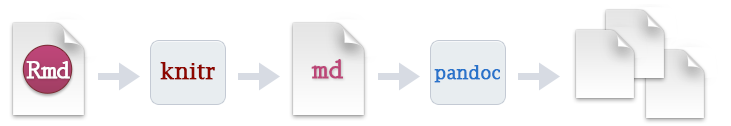
\includegraphics[width=\ScaleIfNeeded]{pictures/RMarkdown}
\caption{RMarkdown Überblick, Quelle: \cite{rmarkdown}}
\label{pic:RMarkdown}
\end{figure}

Der Arbeitsablauf ist ganz einfach, wie in der Abbildung \ref{pic:RMarkdown} zu sehen ist. Nach der Erstellung der RMD-Datei wird mit dem Paket \emph{knitr} der R-Code in der Datei ausgeführt und die Ergebnisse in die resultierende Datei, normale Markdown-Datei (.md Dateiendung), eingefügt. Im Anschluss wird mittels dem Programm \emph{pandoc}, das bereits in das RStudio integriert ist, die Datei in das Ausgabeformat gebracht. Somit lässt sich mit wenigen Schritten, dynamisch erzeugte Daten mittels R-Code, in eine schön formatierte Präsentation im PDF-Format unterbringen. Diesen gesamten Ablauf kapselt das \emph{RMarkdown}-Paket in einen einzigen Funktionsaufruf (\texttt{render}-Funktion). Dadurch wird für den Benutzer der Prozess wesentlich vereinfacht und er kann sich auf das Grundsätzliche, nämlich der Programmierung bzw. der Erstellung der RMD-Datei konzentrieren \cite{rmarkdown}.

Für dynamische Grafiken wurde das Paket Ti\textit{k}Z verwendet, das in \LaTeX integriert wird. Mit dieser Kombination lassen sich schöne Grafiken dynamisch aufbauen mit relativ kompakten Code. Die Klasse Beamer in \LaTeX ermöglicht es Präsentationen zu erzeugen und somit Inhalte mittels verschiedenen Einblendungen darzustellen. Mit dieser Fähigkeit lassen sich auch verschiedene Bereiche in einer Ti\textit{k}Z-Zeichnung hintereinander einblenden, dadurch erhält der Benutzer einen besseren Überblick, wie die Grafik entsteht und kann daraus besser ableiten, wie der Vorgang abgelaufen ist. Diese Tatsache ist vor allem wichtig, wenn sich zukünftige Studenten die Visualisierungsfolien von der Kodierung und Dekodierung anschauen, da dort der genaue Ablauf mit Hilfe von verschiedenen Grafiken erklärt ist. Durch den langsamen Aufbau der Grafiken soll es den Studierenden erleichtert werden, das Prinzip des Turbo-Kode-Verfahrens zu verstehen. Mit dieser visuellen Unterstützung sollen, die in der Vorlesung theoretisch erklärten Abläufe vertieft und praktisch mit den R-Funktionen umgesetzt werden.  